\documentclass[11pt, a4paper]{article}
\usepackage{pdfpages}
\usepackage{parallel}
\usepackage[T2A]{fontenc}
%\usepackage{ucs}
\usepackage[utf8]{inputenc}
\usepackage[english,russian]{babel}
\usepackage{hyperref}
\usepackage{rotating}
\usepackage[inner=2cm,top=1.8cm,outer=2cm,bottom=2.3cm,nohead]{geometry}
%\usepackage{listings}
\usepackage{graphicx}
\usepackage{wrapfig}
\usepackage{longtable}
\usepackage{indentfirst}
\usepackage{array}
\usepackage{tikzsymbols}
\usepackage{soul}
\usepackage[ruled,vlined]{algorithm2e}
\usepackage{qrcode}
\counterwithout{figure}{section} 

\usepackage{url}
\makeatletter
\g@addto@macro{\UrlBreaks}{\UrlOrds}
\makeatother

\newcolumntype{P}[1]{>{\raggedright\arraybackslash}p{#1}}
\frenchspacing
%\usepackage{fixltx2e} %text sub- and superscripts
\usepackage{icomma} % коскі ў матэматычным рэжыме
%\PreloadUnicodePage{4}

\newcommand{\longpage}{\enlargethispage{\baselineskip}}
\newcommand{\shortpage}{\enlargethispage{-\baselineskip}}

\def\switchlang#1{\expandafter\csname switchlang#1\endcsname}
\def\switchlangbe{
\let\saverefname=\refname%
\def\refname{Літаратура}%
\def\figurename{Іл.}%
}
\def\switchlangru{
\let\saverefname=\refname%
\let\savefigurename=\figurename%
\def\refname{Литература}%
\def\figurename{Рис.}%
}
\def\switchlangen{
\let\saverefname=\refname%
\def\refname{References}%
\def\figurename{Fig.}%
}

\hyphenation{admi-ni-stra-tive}
\hyphenation{ex-pe-ri-ence}
\hyphenation{fle-xi-bi-li-ty}
\hyphenation{Py-thon}
\hyphenation{ma-the-ma-ti-cal}
\hyphenation{re-ported}
\hyphenation{imp-le-menta-tions}
\hyphenation{pro-vides}
\hyphenation{en-gi-neering}
\hyphenation{com-pa-ti-bi-li-ty}
\hyphenation{im-pos-sible}
\hyphenation{desk-top}
\hyphenation{elec-tro-nic}
\hyphenation{com-pa-ny}
\hyphenation{de-ve-lop-ment}
\hyphenation{de-ve-loping}
\hyphenation{de-ve-lop}
\hyphenation{da-ta-ba-se}
\hyphenation{plat-forms}
\hyphenation{or-ga-ni-za-tion}
\hyphenation{pro-gramming}
\hyphenation{in-stru-ments}
\hyphenation{Li-nux}
\hyphenation{sour-ce}
\hyphenation{en-vi-ron-ment}
\hyphenation{Te-le-pathy}
\hyphenation{Li-nux-ov-ka}
\hyphenation{Open-BSD}
\hyphenation{Free-BSD}
\hyphenation{men-ti-on-ed}
\hyphenation{app-li-ca-tion}

\def\progref!#1!{\texttt{#1}}
\renewcommand{\arraystretch}{2} %Іначай формулы ў матрыцы зліпаюцца з лініямі
\usepackage{array}

\def\interview #1 (#2), #3, #4, #5\par{

\section[#1, #3, #4]{#1 -- #3, #4}
\def\qname{LVEE}
\def\aname{#1}
\def\q ##1\par{{\noindent \bf \qname: ##1 }\par}
\def\a{{\noindent \bf \aname: } \def\qname{L}\def\aname{#2}}
}

\def\interview* #1 (#2), #3, #4, #5\par{

\section*{#1\\{\small\rm #3, #4. #5}}
\ifx\ParallelWhichBox\undefined%
    \addcontentsline{toc}{section}{#1, #3, #4}%
\else%
\ifnum\ParallelWhichBox=0%
    \addcontentsline{toc}{section}{#1, #3, #4}%
\fi\fi%

\def\qname{LVEE}
\def\aname{#1}
\def\q ##1\par{{\noindent \bf \qname: ##1 }\par}
\def\a{{\noindent \bf \aname: } \def\qname{L}\def\aname{#2}}
}

\newcommand{\interviewfooter}[1]{
\vskip 1em
\noindent \textit{#1}
}

\AtEndDocument{\vfill\centering \qrcode{https://github.com/fiowro/mouses/blob/main/\jobname.pdf}}

\switchlang{en}
\begin{document}

\title{1987 -- Genius GM-5 mouse}
\date{}
\maketitle
\selectlanguage{english}

The GM-5 mouse was released by a Taiwanese company KYE Systems (owner of the Genius brand) for use with Commodore 64 computers (the first mass-produced home computers, which were on the market from 1982 to 1992). The mouse can be dated based on KYE Systems advertising, which mentions the GM-2 (a mouse produced by Z-Nix in 1986 and sold under several brands), the GM-3 (the first mouse produced by KYE itself, in a "new" case relative to the GM-2, with a serial interface and external power supply), and the similar GM-4 without additional power supply \cite{YourComputer}. The GM-6 model, in an even newer case with wide flat buttons, which became the first truly mass-produced Genius mouse (and also the first Genius mouse with a registered FCC ID), dates back to 1987, and its modification GM-6000 dates back to 1988. Thus, the GM-5 mouse is actually a slightly later modification of the GM-3, made for Commodore computers, and could have appeared either in late 1986 or, more likely, in 1987.

\begin{figure}[h]
   \centering
    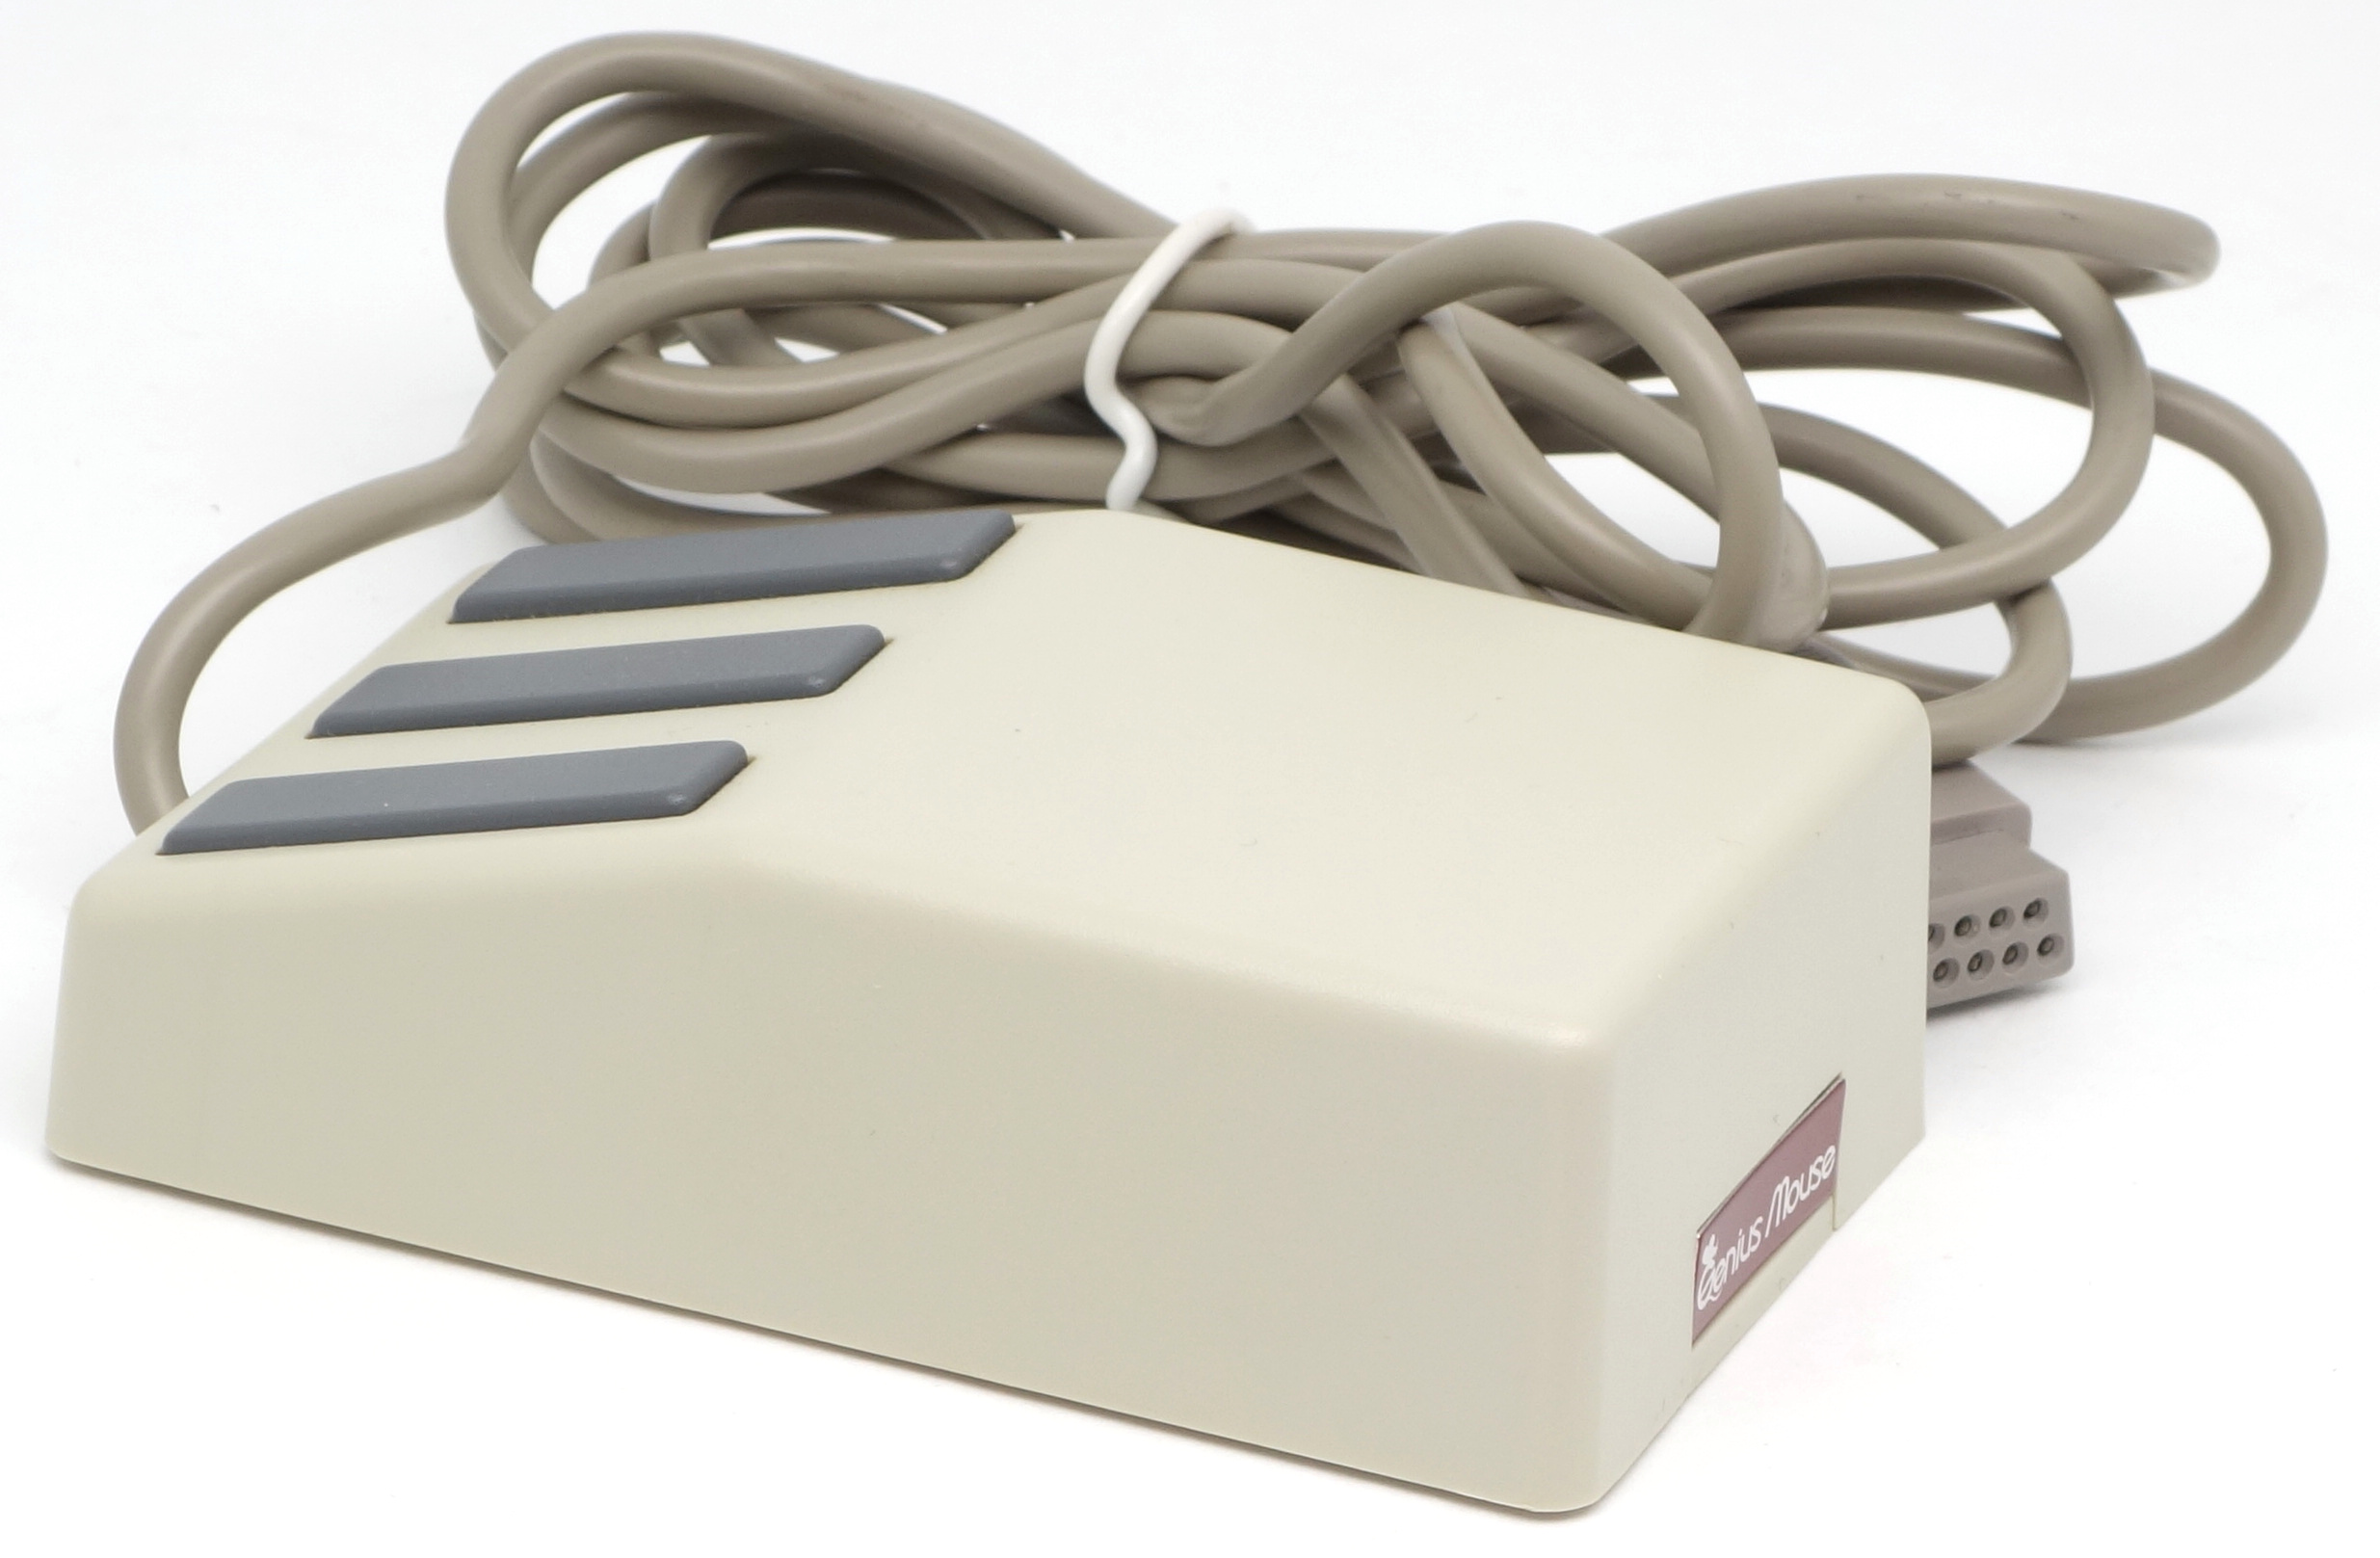
\includegraphics[scale=0.9]{1987_genius_gm5_mouse/pic_30.jpg}
    \caption{Genius GM-5}
    \label{fig:GM5MousePic}
\end{figure}

The mouse is made in a beige case, expressing strict industrial design and minimalism. The case has an almost rectangular shape, if you do not count the forward-slanted part of the upper side, on which there are three elongated rectangular gray buttons. The mouse cable is not provided with protection from mechanical damage at the point where it exits the case. On the bottom (fig. \ref{fig:GM5MouseTopAndBottom}) there is a removable ring made of contrasting gray plastic, designed to remove the ball and clean the mouse (it is attached with a screw -- a design typical of mice from the first half of the 80s). Also on the bottom there are three additional metal balls, which act as supports with a low coefficient of friction.

\begin{figure}[h]
    \centering
    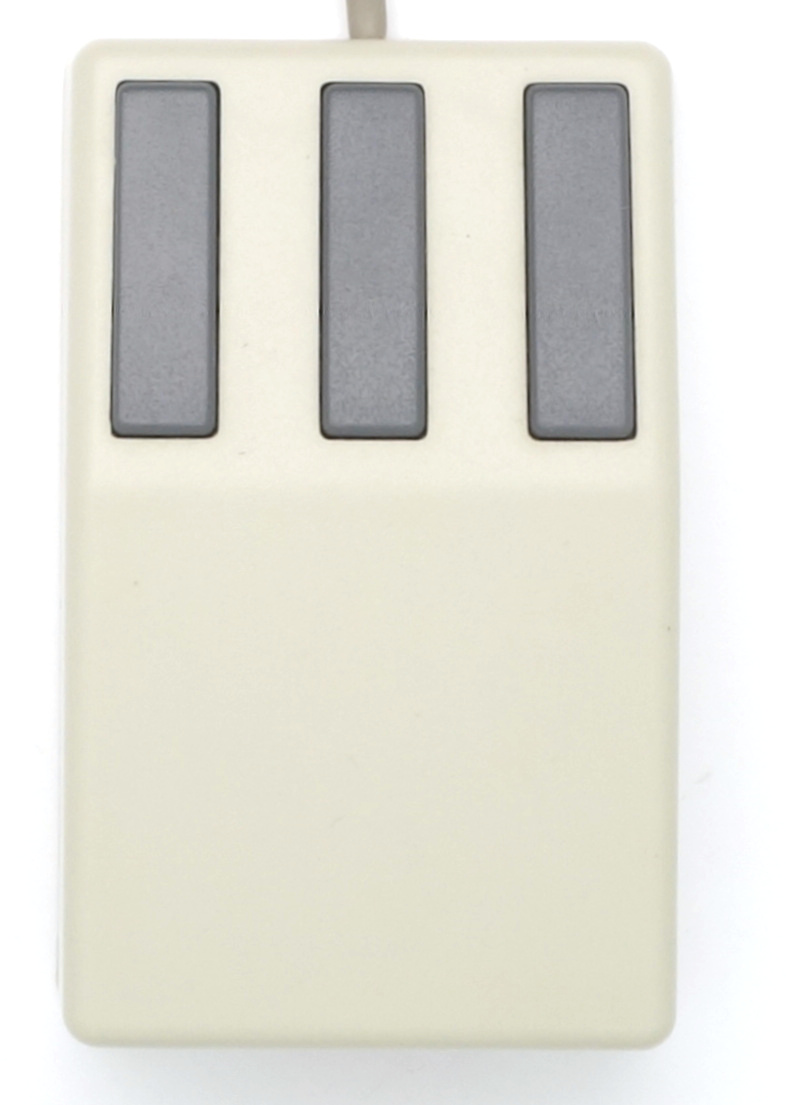
\includegraphics[scale=0.8]{1987_genius_gm5_mouse/top_30.jpg}
    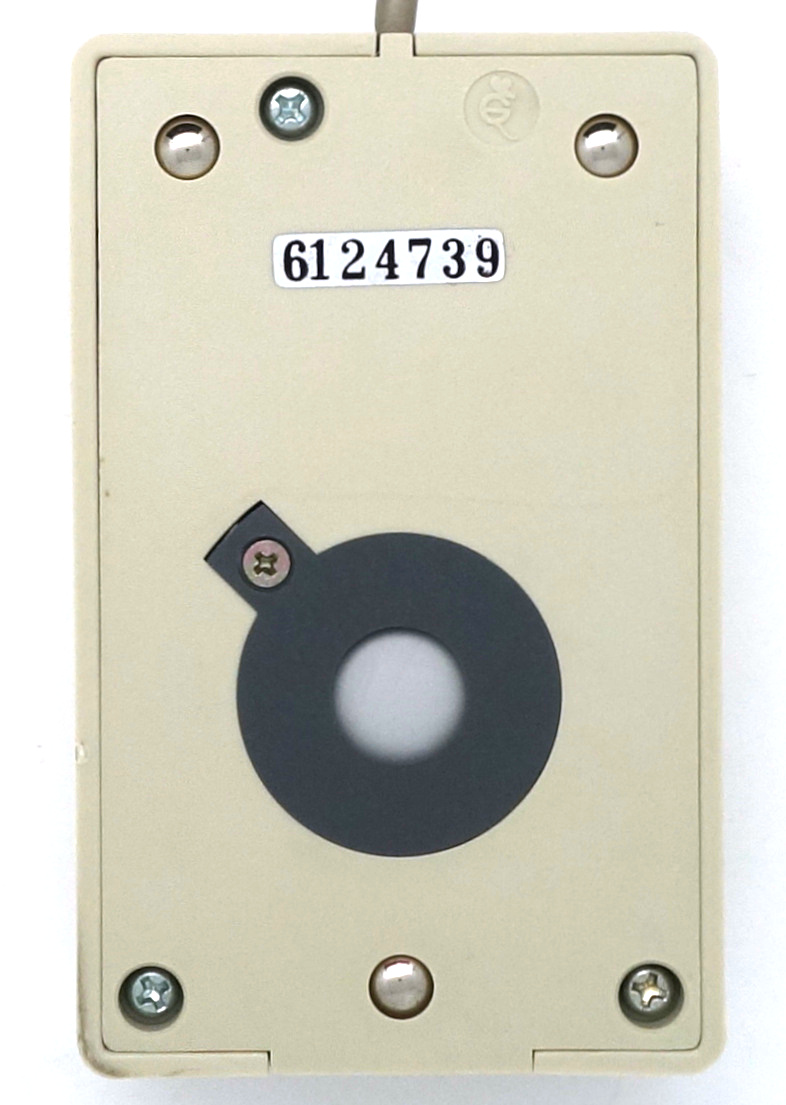
\includegraphics[scale=0.8]{1987_genius_gm5_mouse/bottom_30.jpg}
    \caption{Genius GM-5, top and bottom views}
    \label{fig:GM5MouseTopAndBottom}
\end{figure}

The case is of a size typical for the first half of the 1980s and does not show any identification of the mouse model. Only a metal plate located on the side closest to the user has the inscription ``Genius Mouse'' with the Genius logo inscribed (fig. \ref{fig:GM5MousePic}, \ref{fig:GM5MouseSize}). It should also be noted that the GM-5 mouse was produced for quite a long time, and there are known GM-5 copies in a newer case -- the one in which the GM-6 and GM-6000 \cite{commodore} models appeared. The replacement of the ``old'' case with the ``new'' one in Genius mice occurred gradually: at least the GM-3a (a serial mouse that receives additional power from the keyboard) and GM-4 models can also be found in the new case. The lack of clear identification of the mouse model on the cases allowed KYE Systems to use such case variants as they could, and even alternate them.

\begin{figure}[h]
    \centering
    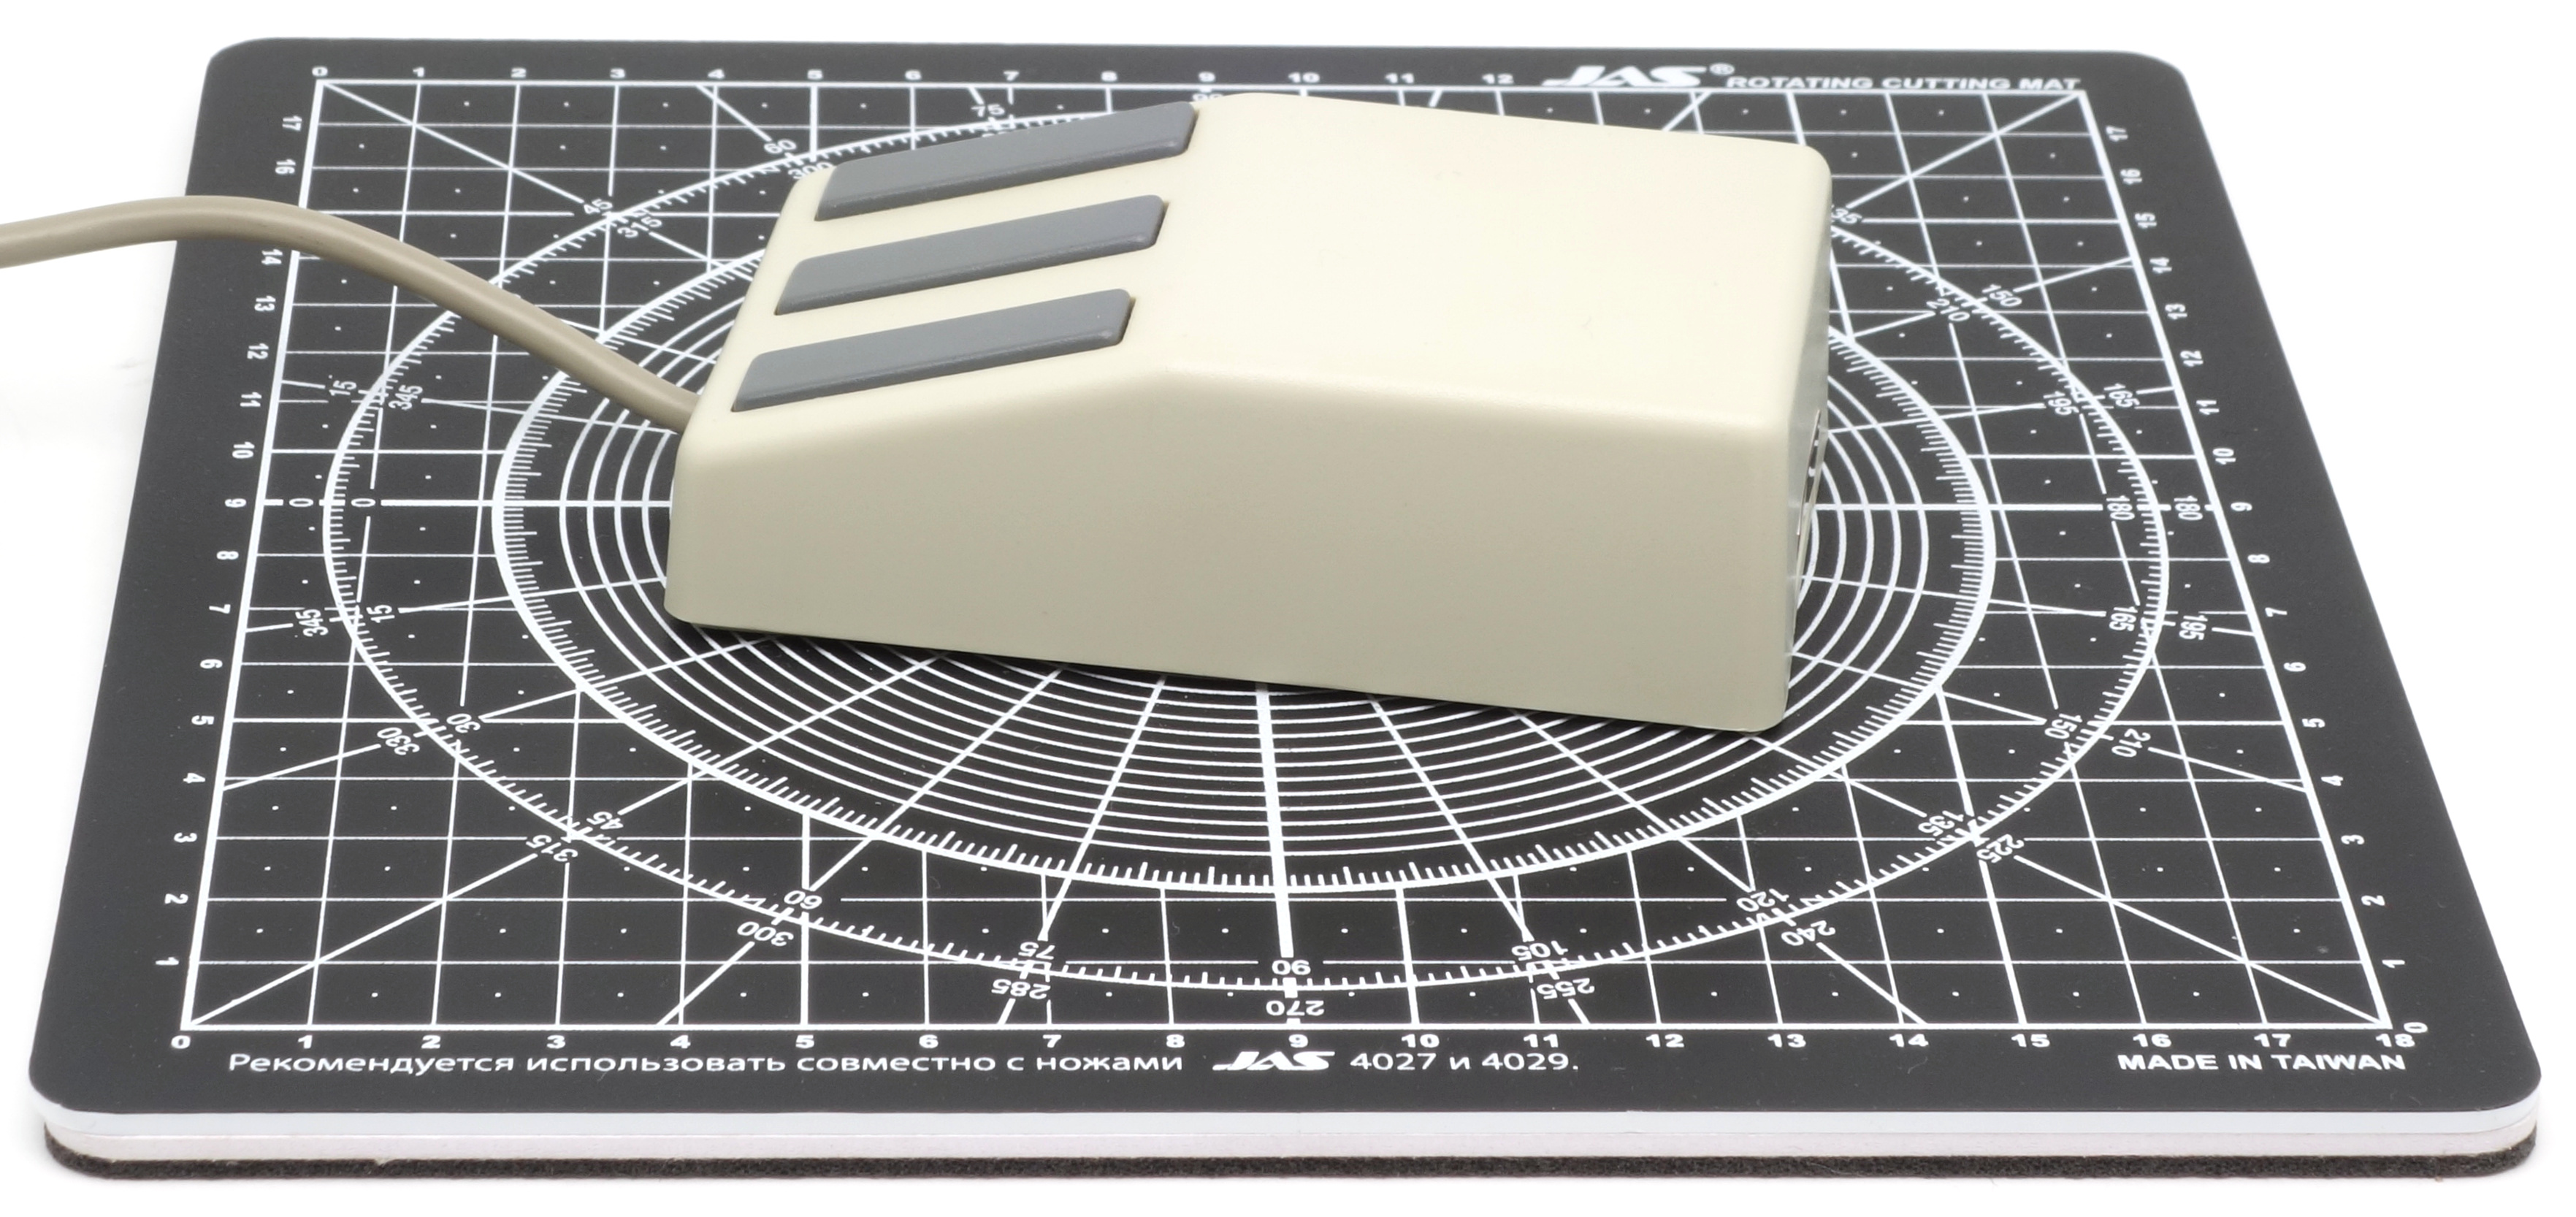
\includegraphics[scale=0.56]{1987_genius_gm5_mouse/size_30.jpg}
    \caption{Genius GM-5 on a graduated pad with a grid step of 1~cm}
    \label{fig:GM5MouseSize}
\end{figure}

In terms of ergonomics, the GM-5 mouse does not have many advantages. The user experience obviously suffers from the severe rectangularity of the body, given that it has a significant height and cannot provide much support for the palm (fig. \ref{fig:GM5MouseHand}).

\begin{figure}[h]
    \centering
    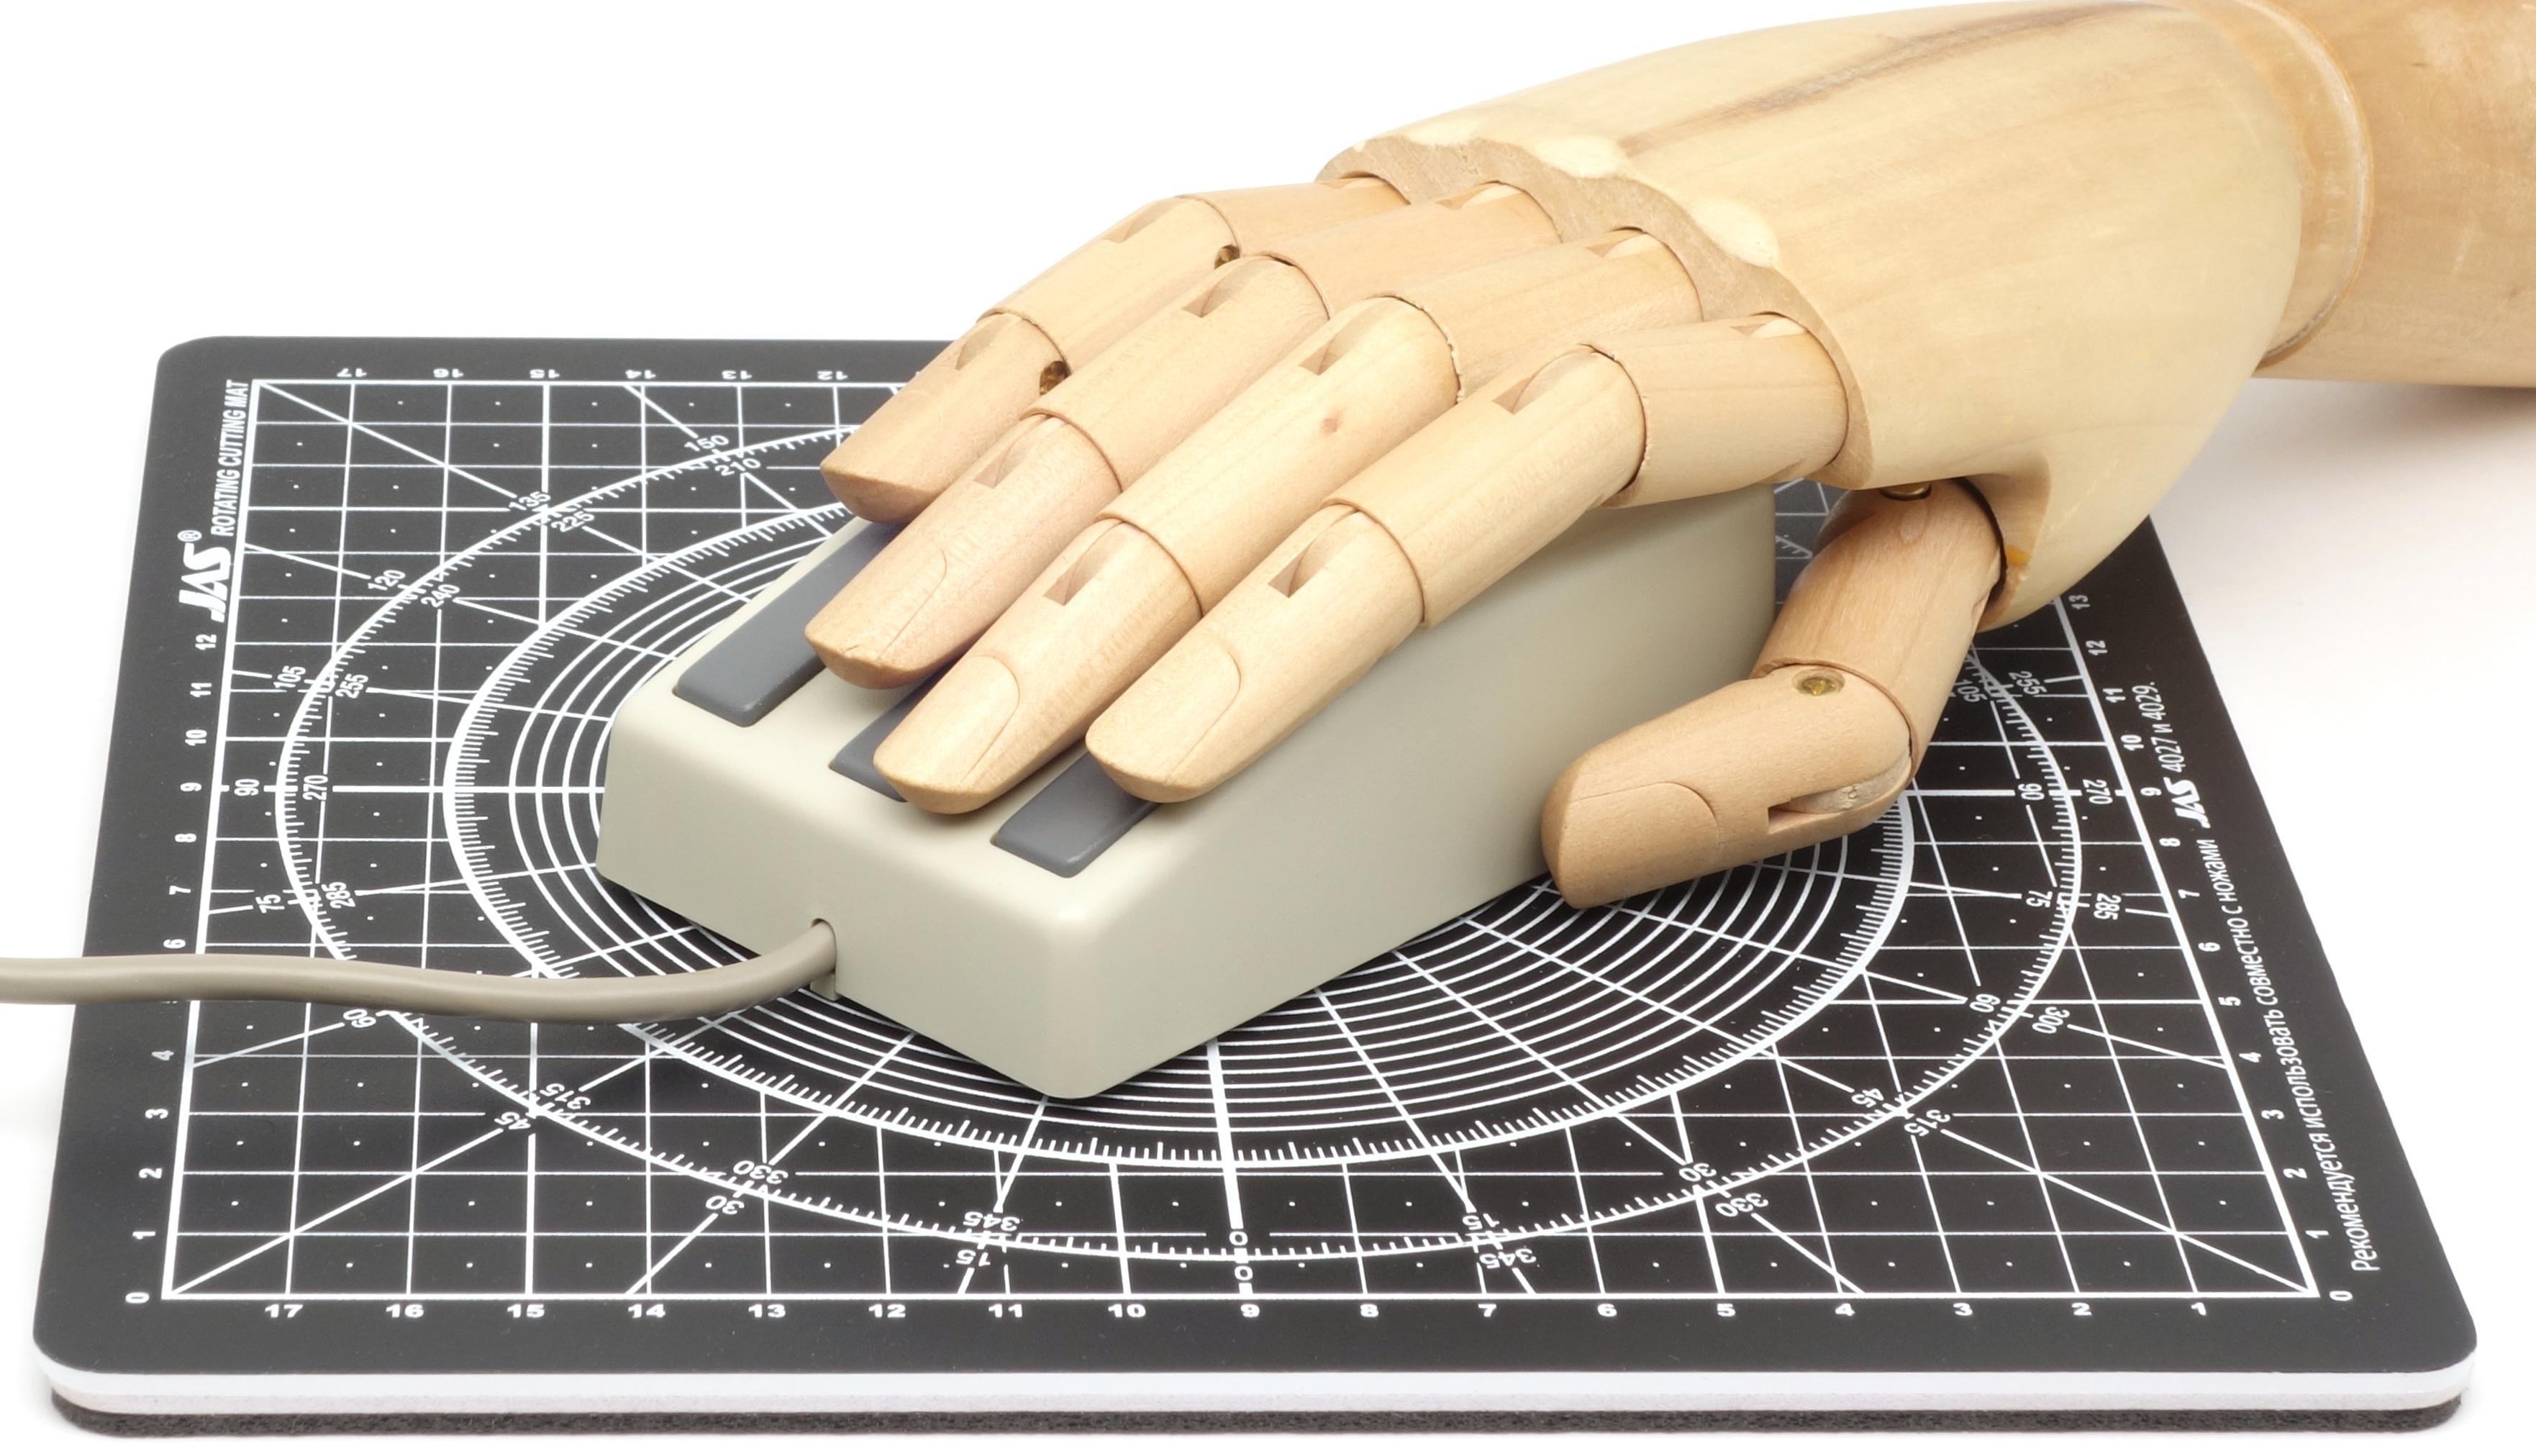
\includegraphics[scale=0.51]{1987_genius_gm5_mouse/hand_30.jpg}
    \caption{Genius GM-5 with a human hand model}
    \label{fig:GM5MouseHand}
\end{figure}

The internal structure of the mouse is shown in fig. \ref{fig:GM5MouseInside}. As you can see, it is an optomechanical design typical of the second half or end of the 80s: with a massive plastic frame covering most of the printed circuit board, and fairly durable brass rollers.

 \begin{figure}[h]
    \centering
    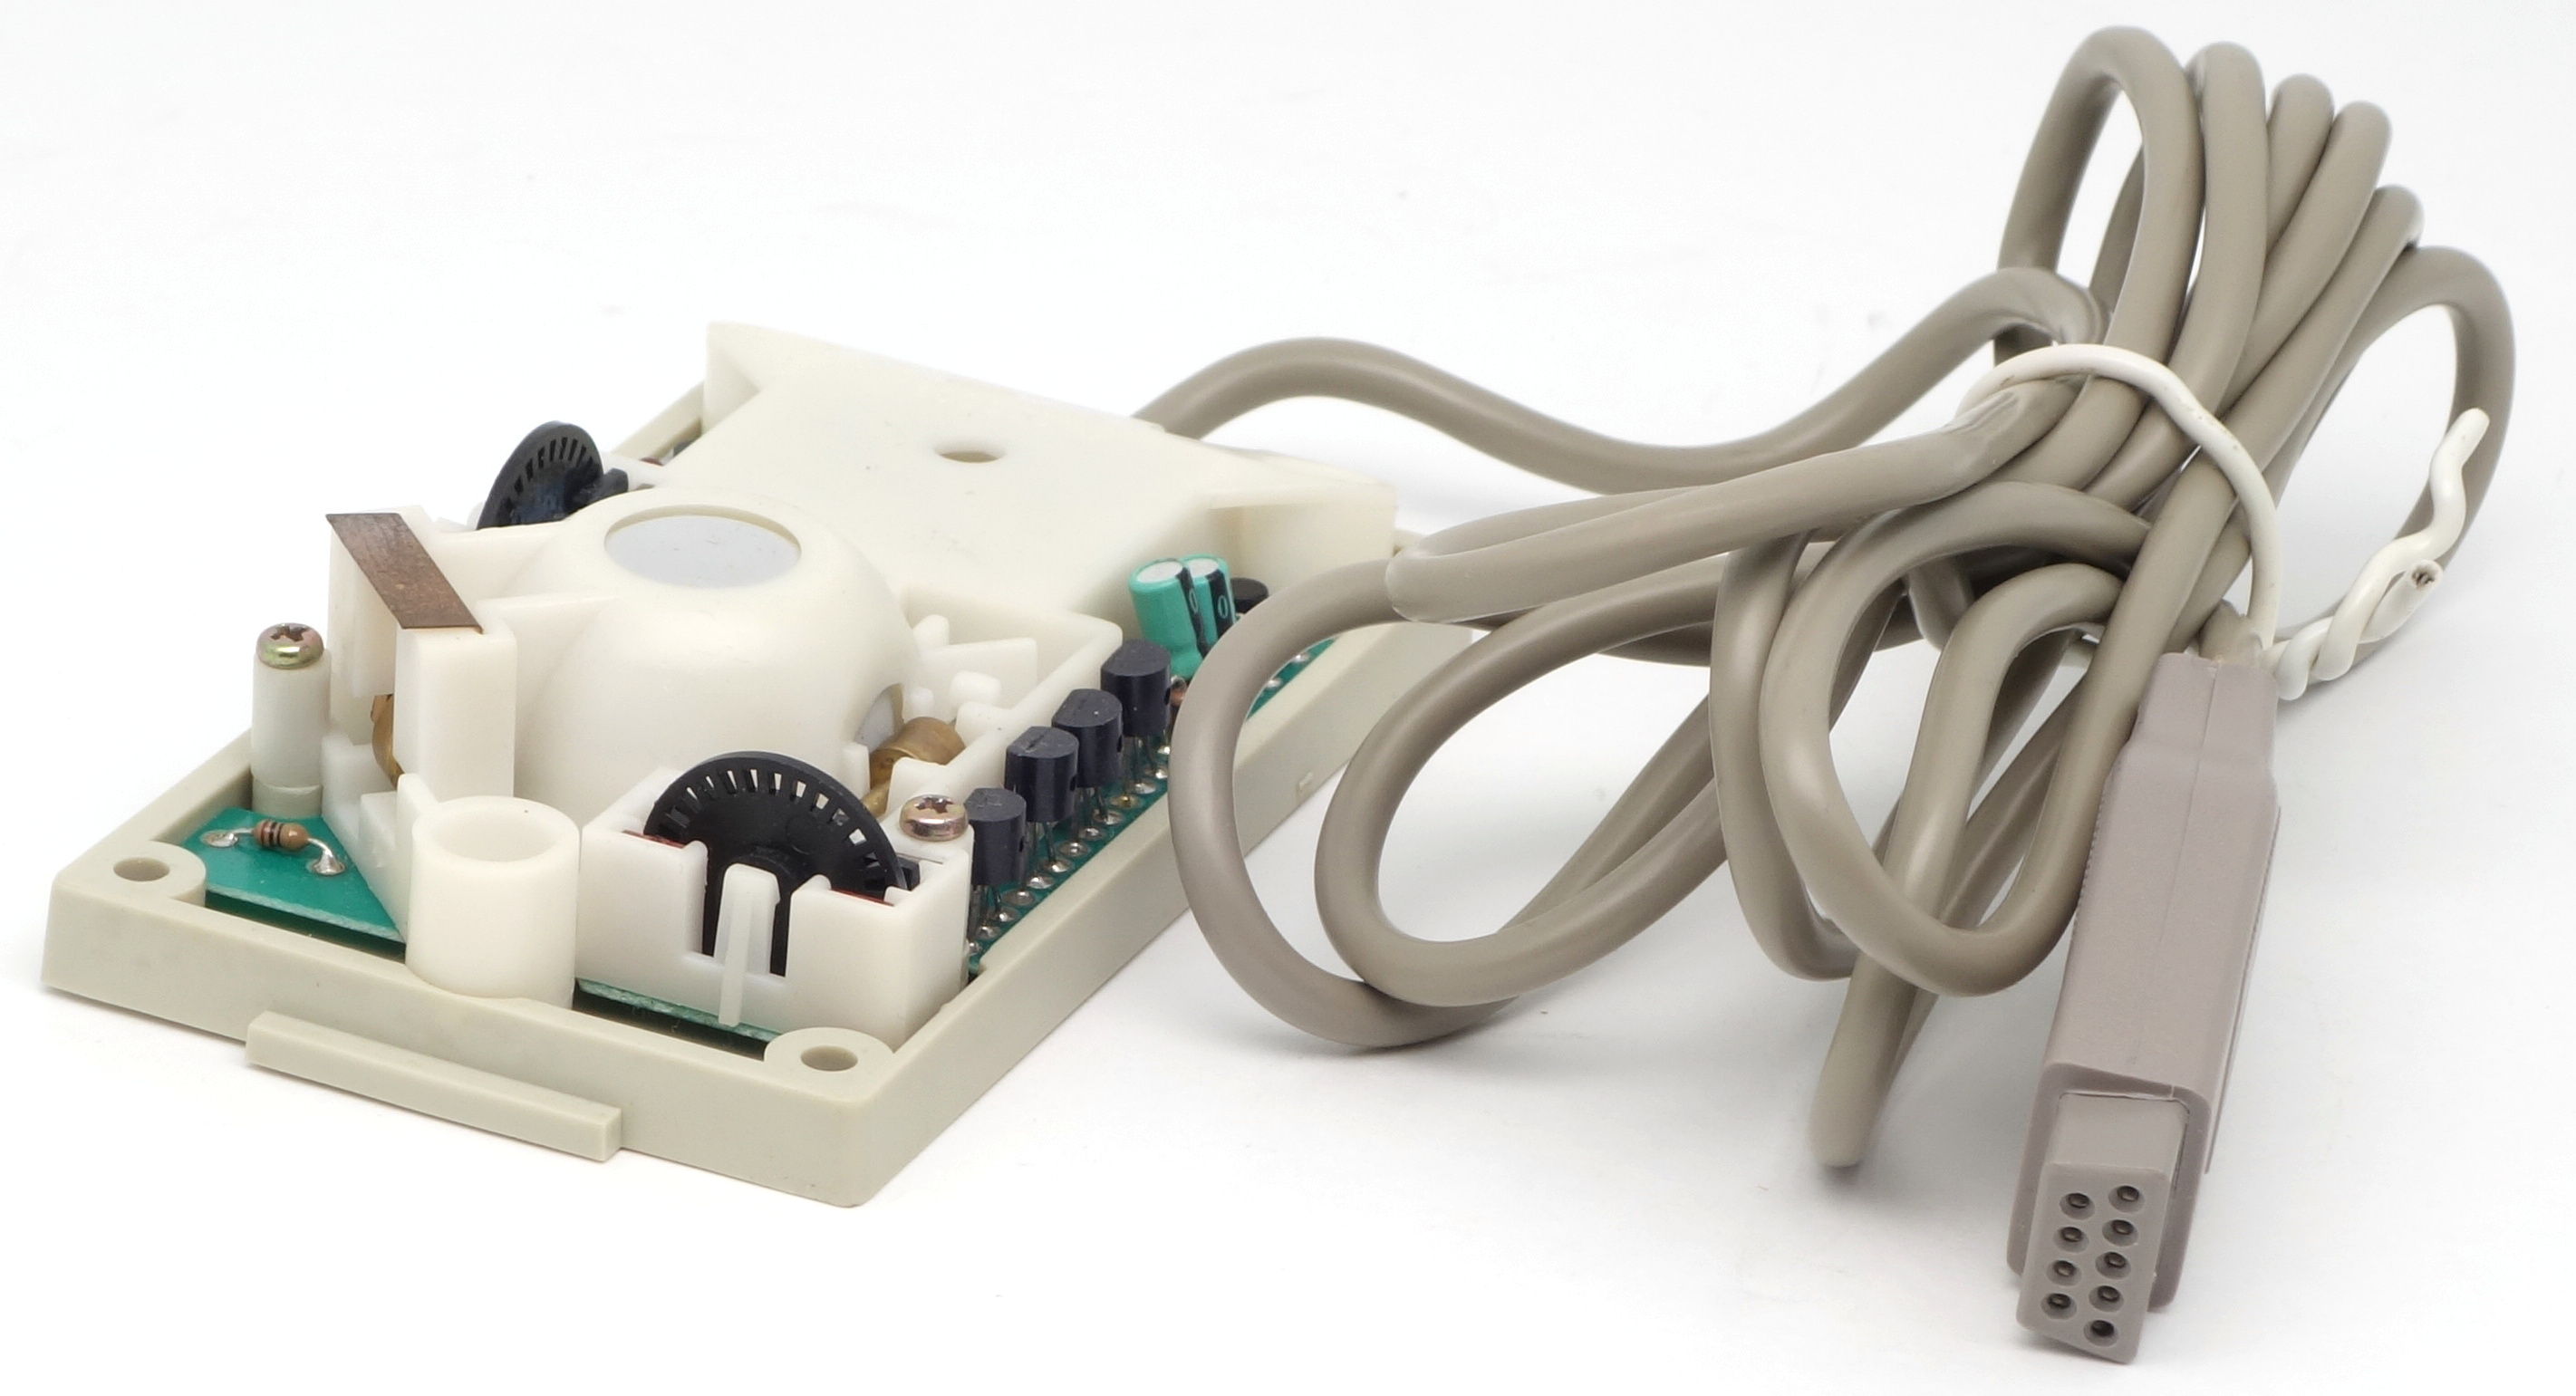
\includegraphics[scale=0.65]{1987_genius_gm5_mouse/inside_30.jpg}
    \caption{Genius GM-5 disassembled}
    \label{fig:GM5MouseInside}
\end{figure}

\begin{thebibliography}{9}
\bibitem {armadale} Mouse - Genius for Commodore 64 | Collections WA \url{https://collectionswa.net.au/items/c38b1405-001b-454e-8b98-e93576187449}
\bibitem {YourComputer} Can Meet All Your Needs. PC/XT/AT. Peripherals \& PC Mouse (adv.) // Your Computer, March 1986. -- P. 24 \url{https://archive.org/details/1986.03-best-buys-ledger-masters/page/24/mode/2up}
\bibitem {commodore} Commodore Info Page - Joystick: Genius Mouse GM-5 [en]. \url{https://www.commodore-info.com/joystick/item/genius_mouse/en/desktop}
\end{thebibliography}
\end{document}
